\documentclass[11pt]{article}

\usepackage[margin=1in]{geometry}
\usepackage[T1]{fontenc}
\usepackage[utf8]{inputenc}
\usepackage{mathptmx}
\usepackage[scaled=0.9]{helvet}
\usepackage{courier}
\usepackage{microtype}
\usepackage{amsmath,amssymb}
\usepackage{booktabs}
\usepackage{tabularx}
\usepackage{array}
\usepackage{enumitem}
\usepackage{xcolor}
\usepackage{algorithm}
\usepackage[noend]{algpseudocode}
\usepackage{tikz}
\usetikzlibrary{positioning,arrows.meta,fit}
\usepackage[numbers,sort&compress]{natbib}
\usepackage[colorlinks=true,linkcolor=blue!50!black,citecolor=blue!50!black,urlcolor=blue!50!black]{hyperref}
\usepackage[capitalise,noabbrev]{cleveref}

\setlist{itemsep=2pt,topsep=4pt}
\newcolumntype{Y}{>{\raggedright\arraybackslash}X}
\newcommand{\stilde}{\tilde{s}}
\newcommand{\splus}{S^{+}}
\newcommand{\code}[1]{\texttt{#1}}

\title{\Large\textbf{OpenReflect: A Fully Specified Recipe and Reference Implementation\\for Training Long-Horizon Self-Improving Agents}}
% TODO(author): add affiliation and contact email on the line below before submitting.
\author{Dulguun Enkhtsatsral}
\date{}

\begin{document}
\maketitle

\begin{abstract}
AREX-2 shows that a 27B-parameter agent trained by imitation on long-horizon improvement trajectories can keep refining a solution for hours, and that this ability transfers to deep-research tasks. The paper describes its training recipe in prose and releases only evaluation code. Several components a reimplementation needs are left open: numeric thresholds for filtering environments and accepting trajectories, a definition of the ``no-progress'' turns excluded from the loss, the agent's tool set, and what happens when a multi-hour run exceeds the context window. We present OpenReflect, a complete specification of this recipe together with an open reference implementation. It contributes (1) a noise-aware environment filter, baseline-to-reference score normalization, benchmark decontamination, and an isolated, hash-checked scorer with a process audit; (2) Round Ledger Compaction (RLC), a context manager that keeps every round, including failures, visible in a structured ledger and freezes the context prefix between compactions, so each segment between compactions is exactly one training window; (3) Progress-Aware Loss Masking (PALM), deterministic rules for redundant, null, and polling turns plus provenance-based credit for turns that lead to score improvements; and (4) a full training configuration. The implementation includes tests that check, among other properties, that every context the agent sends to the model is reproduced exactly by the offline training replay. We define an evaluation protocol on the six AREX-2 benchmarks with seven ablations and process metrics that measure reflection and long-horizon execution directly. This report specifies the method and protocol; experimental results are not yet available.
\end{abstract}

% ===================================================================
\section{Introduction}
% ===================================================================

An agent that can improve its own solution over many rounds converts extra test-time compute into better results. AREX-2~\citep{qian2026arex2} frames this as self-improvement through test-time scaling and splits the gain into two capabilities: \emph{reflection}, which sets the mean gain per productive round, and \emph{long-horizon execution}, which sets how many rounds remain productive. Trained only by imitation on teacher trajectories from machine-learning engineering and competitive-programming environments, AREX-2 reports 81.8 on MLE-bench Lite and 70.7 on Frontier-CS, along with gains on deep-research benchmarks that provide no score feedback.

The result is useful but difficult to build on. The public repository contains evaluation runners only. The paper specifies its pipeline qualitatively: environments are kept when a baseline scores ``well below the reference''; the loss skips ``near-duplicate turns''; trajectories are accepted when the final score is ``high.'' Two questions receive no answer: how a run that lasts up to 12 hours fits in a finite context window, and which teacher model generates the data.

This report does not claim a new capability. Its goal is to make the AREX-2 recipe reproducible and testable. For each component AREX-2 leaves open, we give a precise specification, a rationale, a configuration key, and an ablation that tests whether the choice matters. We also release a reference implementation, built as an extension of the AREX-2 repository, so that each specification can be checked against working code.

\paragraph{Contributions.}
\begin{enumerate}
  \item \textbf{Environment specification} (\cref{sec:envs}): baseline-to-reference normalization, a noise-aware headroom filter, benchmark decontamination, and scorer isolation with a process audit against reward hacking.
  \item \textbf{Round Ledger Compaction} (\cref{sec:rlc}): a context manager for multi-hour runs that keeps a structured record of every round, freezes the context prefix between compactions, and is shared verbatim by the agent and the training data pipeline.
  \item \textbf{Progress-Aware Loss Masking} (\cref{sec:palm}): formal rules for zero-weight turns and a provenance set of full-credit turns, computed deterministically from trajectory logs.
  \item \textbf{A complete recipe and reference implementation} (\cref{sec:recipe,sec:impl}): acceptance rules, every training hyperparameter, configuration files for each ablation, and tests for the properties the method depends on.
  \item \textbf{An evaluation protocol} (\cref{sec:protocol}): seven ablations and five process metrics that measure the two capabilities AREX-2 names, rather than final scores alone.
\end{enumerate}

% ===================================================================
\section{Background and Gap Analysis}
\label{sec:background}
% ===================================================================

\paragraph{The AREX-2 framework.}
In round $t$ the agent submits a solution $y_t$ and receives feedback $f_t$: a score plus logs, errors, and timings. The expected total improvement over $T$ rounds is
\begin{equation}
  \mathbb{E}[\Delta_{\text{total}}] \;=\; \sum_{t=1}^{T} r_t \;\approx\; \bar{r}\cdot T^{*},
  \label{eq:decomp}
\end{equation}
where $\bar{r}$ is the mean gain per productive round and $T^{*}$ is the number of productive rounds. The AREX-2 pipeline has four stages: (i) build environments from GitHub repositories and online judges; (ii) generate long teacher trajectories that keep every round, including regressions; (iii) accept whole trajectories by final score and process conformance; and (iv) fine-tune Qwen3.8-27B~\citep{qwen2026qwen38} with loss only on turns that make progress, mixed with unchanged deep-research data from the AREX recipe~\citep{lu2026arex}.

\paragraph{What is unspecified.}
\Cref{tab:gaps} lists each component that the paper or its repository leaves open, and where this report addresses it. We add one further check that AREX-2 does not run. Its claim that gains transfer across domains rests on holding the deep-research data fixed. That design does not separate the effect of iterative trajectory structure from the effect of additional agentic training tokens. Ablation A7 (\cref{sec:protocol}) adds a token-matched control.

\begin{table}[t]
\centering
\small
\caption{Components of the AREX-2 recipe that are unspecified, and where OpenReflect specifies them.}
\label{tab:gaps}
\begin{tabularx}{\linewidth}{@{}l Y Y l@{}}
\toprule
Component & Stated in AREX-2 & Missing & Here \\
\midrule
Environment filter & Baseline ``well below the reference'' & Numeric margin; score noise & \S\ref{sec:filter} \\
Score scale & Graded scores ``where possible'' & Normalization across metrics & \S\ref{sec:normalize} \\
Contamination & Not discussed & Overlap with evaluation tasks & \S\ref{sec:decontam} \\
Process conformance & Process must conform & Concrete checks & \S\ref{sec:audit} \\
Agent scaffold & Tool calls, submission, feedback & Tool set; scaffold code & \S\ref{sec:tools} \\
Context management & Failures stay in context; 12\,h runs & Behavior on overflow & \S\ref{sec:rlc} \\
Loss masking & No loss on polling, empty calls, near-duplicates & Detection rules; ``progress'' & \S\ref{sec:palm} \\
Acceptance & Best score above a relative threshold & Values; minimum rounds & \S\ref{sec:accept} \\
Teacher model & ``A teacher model'' & Identity; sensitivity & \S\ref{sec:teacher} \\
Training & Base model; data mix & All hyperparameters & \S\ref{sec:hparams} \\
Released code & Evaluation only & Synthesis, scaffold, training & \S\ref{sec:impl} \\
\bottomrule
\end{tabularx}
\end{table}

\begin{figure}[t]
\centering
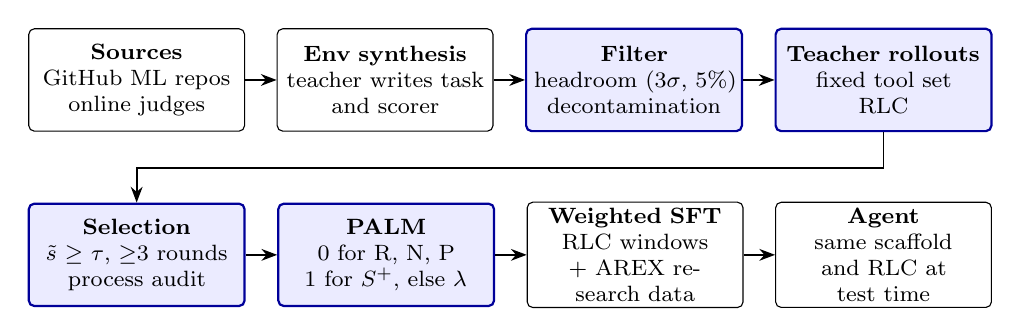
\begin{tikzpicture}[
  node distance=4mm and 4mm,
  box/.style={draw, rounded corners=2pt, align=center, font=\footnotesize, minimum height=13mm, text width=26mm, inner sep=2pt},
  new/.style={box, fill=blue!8, draw=blue!60!black, line width=0.8pt},
  arr/.style={-{Stealth[length=2mm]}, semithick}
]
\node[box] (src) {\textbf{Sources}\\GitHub ML repos\\online judges};
\node[box, right=of src] (syn) {\textbf{Env synthesis}\\teacher writes task\\and scorer};
\node[new, right=of syn] (fil) {\textbf{Filter}\\headroom ($3\sigma$, 5\%)\\decontamination};
\node[new, right=of fil] (roll) {\textbf{Teacher rollouts}\\fixed tool set\\RLC};
\node[new, below=9mm of src] (sel) {\textbf{Selection}\\$\stilde\ge\tau$, $\ge$3 rounds\\process audit};
\node[new, right=of sel] (palm) {\textbf{PALM}\\0 for R, N, P\\1 for $\splus$, else $\lambda$};
\node[box, right=of palm] (sft) {\textbf{Weighted SFT}\\RLC windows\\+ AREX research data};
\node[box, right=of sft] (agent) {\textbf{Agent}\\same scaffold\\and RLC at test time};
\draw[arr] (src) -- (syn); \draw[arr] (syn) -- (fil); \draw[arr] (fil) -- (roll);
\draw[arr] (roll.south) -- ++(0,-4.5mm) -| (sel.north);
\draw[arr] (sel) -- (palm); \draw[arr] (palm) -- (sft); \draw[arr] (sft) -- (agent);
\end{tikzpicture}
\caption{The OpenReflect pipeline. Shaded stages contain components that are new relative to AREX-2; the others follow AREX-2 and are now fully specified. The same scaffold and context manager are used for teacher rollouts, for building training windows, and at test time.}
\label{fig:pipeline}
\end{figure}

% ===================================================================
\section{Environments}
\label{sec:envs}
% ===================================================================

OpenReflect uses the same two environment sources as AREX-2. For \emph{ML repositories}, a candidate must have a permissive license, a runnable entry point, a quantitative metric already computed in its code, and a full run under 2 GPU-hours on one 80\,GB GPU. A teacher model reads a digest of the repository and drafts a task statement asking for the metric to be improved, a deterministic held-out split, a scoring script, a baseline command, and a reference command. For \emph{online-judge problems}, we prefer graded scoring: optimization problems scored against the best known value, or problems with many hidden tests scored by the fraction passed.

\subsection{Normalized score}
\label{sec:normalize}
Raw metrics differ in scale and direction. For environment $e$ with baseline score $b_e$ (a simple solution such as a default configuration, majority class, or brute force) and reference score $s_{\text{ref},e}$ (the mean of $k$ seeded runs), every score is mapped to
\begin{equation}
  \stilde \;=\; \frac{s - b_e}{s_{\text{ref},e} - b_e},
  \label{eq:norm}
\end{equation}
with all three quantities negated when lower is better. The baseline maps to 0 and the reference to 1. Run-to-run noise on this scale is $\varepsilon_e = \sigma_e / |s_{\text{ref},e} - b_e|$, where $\sigma_e$ is the standard deviation of the reference runs; $\varepsilon_e$ is used below to decide whether a change in score is real.

\subsection{Noise-aware headroom filter}
\label{sec:filter}
AREX-2 requires the baseline to score ``well below'' the reference. We run the reference $k=3$ times and keep an environment only if
\begin{equation}
  s_{\text{ref},e} - b_e \;\ge\; \max\!\big(3\,\sigma_e,\; 0.05\,|s_{\text{ref},e}|\big).
  \label{eq:headroom}
\end{equation}
The $3\sigma_e$ term ensures that improvement on the normalized scale is a real signal rather than seed noise. The 5\% term rejects environments whose headroom is statistically significant but too small to support many productive rounds. For judge problems scored by pass fraction we instead require $b_e \le 0.6$ and $s_{\text{ref},e} \ge 0.95$. Both margins are swept in ablation A4.

\subsection{Decontamination}
\label{sec:decontam}
GitHub ML repositories can overlap with Kaggle competitions in MLE-bench~\citep{chan2025mlebench}, and judge problems can overlap with Frontier-CS~\citep{mang2025frontiercs}. An environment is dropped if, against any evaluation task, it shares a dataset (normalized URL, normalized name, or file hash), shares a competition or problem identifier, or has 13-gram overlap of at least 50\% between task statements, following the n-gram check of \citet{brown2020gpt3}. We report the number of environments each rule removes. Ablation A6 measures how much of the final score depends on this step.

\subsection{Scorer isolation and process audit}
\label{sec:audit}
AREX-2 accepts trajectories only if the process conforms to the task requirements, without stating how this is checked. Verifiable environments invite reward hacking~\citep{skalse2022rewardhacking}, so we enforce conformance by construction and then audit it.
\begin{enumerate}
  \item The held-out split and scoring script live in a scorer directory that is never mounted in the agent's sandbox. The agent sees only a public development split and a \code{submit} tool.
  \item Before every run the scorer verifies the SHA-256 hash of its own script and scores a frozen copy of the solution. In container mode the solution is mounted read-only and the scorer has no network access.
  \item For judge problems, 10\% of hidden tests are canaries generated after the trajectory is collected. A solution whose pass rate on regular tests exceeds its pass rate on canaries by more than 0.2 is flagged as overfit.
  \item Rule checks flag reads of paths outside the workspace or inside the scorer directory, hidden-test outputs embedded as literals in the final solution (one output of at least 32 characters, or three of at least 8), and fetches of the source repository's reference solution.
  \item An optional LLM auditor reviews the final diff for metric gaming, such as changing the evaluation split.
\end{enumerate}
A trajectory flagged by any of steps 3 to 5 is rejected.

% ===================================================================
\section{Agent Scaffold and Round Ledger Compaction}
\label{sec:rlc}
% ===================================================================

\subsection{Tool set}
\label{sec:tools}
AREX-2 does not list its tools. We fix one set for all environments so that trajectories share an action space (\cref{tab:tools}). The blocking \code{wait\_job} tool is a deliberate change: in AREX-2, polling turns are generated and then masked out of the loss; a blocking wait removes most of them at the source, which saves context and wall-clock time.

\begin{table}[t]
\centering
\small
\caption{The fixed tool set.}
\label{tab:tools}
\begin{tabularx}{\linewidth}{@{}l Y@{}}
\toprule
Tool & Behavior \\
\midrule
\code{bash} & Shell command in the sandbox; 10-minute timeout; output truncated to about 8K tokens, keeping head and tail. \\
\code{read\_file}, \code{edit\_file} & Inspect and change files. Edits require a unique match and return a unified diff, which PALM uses for provenance. \\
\code{run\_job}, \code{wait\_job} & Start a long command; block until it finishes or a timeout (at most 30 minutes) passes, returning only new log lines. \\
\code{web\_search}, \code{web\_fetch} & Find papers, documentation, and libraries. Disabled where a benchmark forbids it. \\
\code{submit} & Score the current solution. Requires a \code{hypothesis} and a one-line \code{lesson}. Ends the round. \\
\code{answer} & Final answer for research tasks. \\
\bottomrule
\end{tabularx}
\end{table}

\subsection{The overflow problem}
A 12-hour run with hundreds of tool calls produces far more tokens than a context window holds. AREX-2 states that failures and regressions remain in the context, but not what happens when it is full. Truncating the oldest turns removes the early failures the model is meant to learn from; free-form summarization loses scores and error signatures.

\subsection{Round ledger}
The scaffold keeps a \emph{round ledger} with one entry per submission. Most fields are filled automatically: round number, elapsed time, a diff summary of the round's edits, raw score, normalized score, change relative to the best so far, and the first error line of a failed run. The agent writes only two fields, the \code{hypothesis} and \code{lesson} arguments of \code{submit}. Each new entry is also appended to the \code{submit} observation, so the model sees it immediately. When the ledger exceeds a token cap, its oldest non-best entries are merged into one line per strategy family, recording their rounds, best score, number of failures, and recent lessons. No round is deleted, so the AREX-2 principle that failures stay visible holds for runs of any length. For research tasks without a scorer, entries record a candidate answer, a confidence, and evidence URLs instead of a score.

\subsection{Compaction with a frozen prefix}
The context consists of a \emph{prefix} (system prompt, task statement, skills, current best, and the rendered ledger) followed by the verbatim turns of recent rounds. \Cref{alg:rlc} gives the procedure. The prefix is rendered at the start of a run and re-rendered only when a compaction occurs. Between compactions the context therefore grows only by appending turns. This has two consequences. First, key-value caches remain valid across turns. Second, and more important for training, every segment between two compactions is a single sequence that covers all of its turns, which makes the training windows of \cref{sec:windows} exact rather than approximate.

\begin{algorithm}[t]
\caption{Round Ledger Compaction: building the context for the next turn}
\label{alg:rlc}
\begin{algorithmic}[1]
\Require window $W$, threshold $\theta$, rounds kept $K$, ledger cap $L$; current round $r$
\State \textbf{if} prefix is unset \textbf{then} prefix $\gets$ \Call{Render}{pinned, ledger}
\State $C \gets$ prefix $\Vert$ visible turns
\If{$|C| \le \theta W$} \Return $C$ \Comment{no event: context only grew}
\EndIf
\State $c' \gets r - K + 1$
\If{$c' \le c$ \textbf{and} $|\text{ledger}| \le L$ \textbf{and} $|C| \le W$} \Return $C$ \Comment{nothing to compact yet}
\EndIf
\State $c \gets \max(c, c')$ \Comment{turns from rounds $< c$ are now ledger-only}
\State \textbf{if} $|\text{ledger}| > L$ \textbf{then} merge oldest non-best entries per strategy family
\State prefix $\gets$ \Call{Render}{pinned, ledger} \Comment{includes a note that rounds $1..c{-}1$ were compacted}
\State $C \gets$ prefix $\Vert$ visible turns
\While{$|C| > W$ \textbf{and} more than one visible turn} drop the oldest visible turn
\EndWhile
\State record a compaction event; \Return $C$
\end{algorithmic}
\end{algorithm}

Defaults are $W=128\text{K}$ tokens, $\theta=0.75$, $K=2$, and $L=16\text{K}$ tokens. The final loop is a guard for a single round that alone exceeds the window.

\subsection{Identical contexts at training and test time}
\label{sec:windows}
A model trained on uncompacted trajectories but run with compaction sees a context distribution it was never trained on. We avoid this by construction: one context-building component is used by the live agent and by the offline training replay. Tool-call identifiers are deterministic (\code{call\_}$i$ for turn $i$), so the replay emits the same messages byte for byte. The teacher runs with RLC during collection, so its decisions are conditioned on the same views. To build training data, each accepted trajectory is replayed; every compaction event starts a new window whose prefix is the compacted context at that moment, and the turns that follow are appended until the next event. Loss is applied only to assistant turns inside the window, weighted by PALM. The reference implementation tests this property directly (\cref{sec:impl}).

% ===================================================================
\section{Progress-Aware Loss Masking}
\label{sec:palm}
% ===================================================================

AREX-2 applies loss to ``decisions that move the solution forward'' and none to ``repeated polling, calls that return no new observation, and near-duplicate turns,'' without saying how these are detected. PALM turns these descriptions into deterministic rules over the trajectory log, so masks can be reproduced and audited.

\paragraph{Setup.}
A trajectory has assistant turns $a_1,\dots,a_N$, each consisting of reasoning and one tool call, followed by an observation $o_i$. After each turn the scaffold records a hash $h_i$ of the workspace. Let $B_t$ be the best normalized score after round $t$, with $B_0 = 0$ (the baseline). A submission at round $t$ is \emph{improving} if $\stilde_t > B_{t-1} + \varepsilon_e$.

\subsection{Zero-weight turns}
A turn receives weight 0 if any of the following holds.
\begin{itemize}
  \item \textbf{Redundant}, $R(i)$: some earlier turn $j$ in the last $W_R = 20$ turns has a near-identical canonical action (tool name and arguments with whitespace normalized; Jaccard similarity of word 5-gram shingles $\ge 0.9$), and the workspace has not changed since turn $j$, including by turn $i$ itself. Re-running a training script after an edit is therefore a new experiment, not a duplicate. Status checks are excluded from $R$ and handled by $P$, because a repeated status check can return new information.
  \item \textbf{Null observation}, $N(i)$: after normalization (removing timestamps, process IDs, durations, ANSI codes, and progress-bar lines) the observation is empty with the workspace unchanged, or identical to the last observation from the same tool on the same target with the workspace unchanged.
  \item \textbf{Polling}, $P(i)$: a status-only call (for example \code{wait\_job} returning on timeout, \code{ps}, \code{nvidia-smi}, or \code{tail} on a log) that adds no new log lines since the last status call on the same target.
\end{itemize}
System messages, observations, and retrieved documents also receive no loss, as in AREX-2.

\subsection{Full-credit turns}
A turn joins the provenance set $\splus$ if any of the following holds.
\begin{enumerate}
  \item \emph{Surviving edit}: it is an \code{edit\_file} turn and at least one of its diff hunks appears line for line (ignoring blank lines and trailing whitespace) in the solution scored at a later improving submission. A deletion-only hunk survives if the removed block is still absent. This approximates \code{git blame} without requiring repository history.
  \item \emph{Improving submission}: it is the \code{submit} call of an improving round.
  \item \emph{Supporting evidence}: it is a read, search, fetch, or inspection turn within 50 turns before a turn from rule 1 or 2, and the later turn uses it: the two share a file path, URL, or identifier, or an 8-gram of the observation appears in the later turn's reasoning. Paths and identifiers that occur in the task statement are excluded, since every file the task names would otherwise qualify. Only one hop is followed.
  \item \emph{Recovery}: it is the first edit after a regression ($\stilde_t < B_{t-1} - \varepsilon_e$) or a failed submission, it touches the file named in the error if one is named, and the agent regains at least $B_{t-1}$ within $M=3$ rounds. This credits diagnosis and repair even when the repaired code is later replaced.
\end{enumerate}

\subsection{Weights and loss}
All remaining turns receive weight $\lambda$. These are plausible steps that did not lead to a gain, such as a reasonable experiment that failed. The AREX-2 description implies $\lambda=0$ for some of them, yet trajectories are accepted without filtering rounds so that the model learns to explore. We therefore treat $\lambda$ as an open question, default to $\lambda = 0.5$, and sweep it in ablation A1:
\begin{equation}
  w_i =
  \begin{cases}
    0 & \text{if } R(i) \lor N(i) \lor P(i),\\
    1 & \text{if } i \in \splus,\\
    \lambda & \text{otherwise.}
  \end{cases}
  \label{eq:weights}
\end{equation}
The loss is a weighted token-level cross-entropy normalized by the weighted token count, so that long trajectories do not dominate a batch:
\begin{equation}
  \mathcal{L}(\theta) \;=\; -\,\frac{\sum_{i} w_i \sum_{k \in a_i} \log p_\theta(x_k \mid x_{<k})}{\sum_{i} w_i\, |a_i|}.
  \label{eq:loss}
\end{equation}
Reasoning tokens inside a turn share the turn's weight.

\subsection{Checking the rules}
Heuristic rules can be wrong, so we measure them before training. Two annotators label 500 turns sampled from 50 trajectories as \emph{no progress}, \emph{neutral}, or \emph{progress}. We report precision and recall of the zero-weight rules and of $\splus$ against these labels, Cohen's $\kappa$ between the rules and the adjudicated labels, and $\kappa$ between the two annotators. If the rules agree with the labels less than the annotators agree with each other, thresholds are revised before any training run.

% ===================================================================
\section{Trajectory Selection and Training Recipe}
\label{sec:recipe}
% ===================================================================

\subsection{Acceptance rule}
\label{sec:accept}
As in AREX-2, whole trajectories are accepted or rejected and individual rounds are never filtered. A trajectory is accepted if (i) its best normalized score satisfies $\stilde_{\text{best}} \ge \tau_d$, with $\tau_{\text{ML}} = 0.9$ and $\tau_{\text{judge}} = 0.95$; (ii) it has at least 3 scored rounds; (iii) at least one round after the first is improving, so every accepted trajectory shows iteration; and (iv) the process audit raised no flag. At most two trajectories are kept per environment, preferring higher best scores, so that easy environments do not dominate. Ablation A3 sweeps $\tau \in \{0.7, 0.9, 1.0\}$.

\subsection{Teacher model}
\label{sec:teacher}
AREX-2 does not name its teacher, although results may depend heavily on it. We select the teacher with a pilot: each candidate runs on 50 held-out environments, and we choose the one with the most accepted trajectories per GPU-hour. We prefer an open-weight teacher so that trajectories can be redistributed under its license. The teacher and version will be reported with results. Ablation A5 retrains with the runner-up teacher.

\subsection{Data and hyperparameters}
\label{sec:hparams}
\Cref{tab:hparams} lists the planned data scale and the training configuration. These are proposed defaults chosen to match common practice for full-parameter supervised fine-tuning at this scale; they will be tuned on a validation split of 100 environments, and any changes will be reported.

\begin{table}[t]
\centering
\small
\caption{Planned data scale and training configuration (proposed defaults, not tuned values).}
\label{tab:hparams}
\begin{tabularx}{\linewidth}{@{}l Y@{}}
\toprule
Item & Value \\
\midrule
Environments after filtering & 2{,}000 (1{,}200 ML, 800 judge) \\
Teacher rollouts & 4 per environment, temperature 0.7 \\
Rollout budget & 12\,h (ML) or 5\,h (judge); at most 400 tool calls \\
Deep-research data & AREX recipe data, unchanged; default token ratio 1:1 \\
\midrule
Base model & Qwen3.8-27B (as in AREX-2) \\
Method & Full-parameter SFT with PALM weights; no reinforcement learning \\
Context & 128K tokens, RLC windows (\cref{sec:windows}) \\
Optimizer & AdamW, $\beta = (0.9, 0.95)$, weight decay 0.1 \\
Learning rate & Peak $10^{-5}$, 3\% linear warmup, cosine decay to $10^{-6}$ \\
Epochs; global batch & 2; 64 windows \\
Gradient clipping & 1.0 \\
Precision; parallelism & bf16; ZeRO-3 with sequence parallelism \\
Seeds & 3 for the main model, 1 per ablation \\
\bottomrule
\end{tabularx}
\end{table}

% ===================================================================
\section{Reference Implementation}
\label{sec:impl}
% ===================================================================

We release the implementation as an extension of the AREX-2 repository, whose evaluation harness is kept unchanged. The package has six modules: \code{envs} (normalization, filter, decontamination, scorer, audit, synthesis), \code{scaffold} (tools, sandboxes, ledger, RLC, shared context builder, agent loop), \code{palm} (rules, provenance, weights, validation), \code{selection}, \code{train} (window construction and the weighted loss of \cref{eq:loss}), and \code{metrics}. A command-line tool runs each pipeline stage, and every threshold in this report is a configuration value. Each ablation in \cref{tab:ablations} is a configuration file that inherits the defaults and overrides only what it changes.

The test suite checks the properties the method depends on, including: normalization for both metric directions; each filter and decontamination rule; that the scorer refuses to run when its script hash changes; each audit rule; that ledger compaction never drops a round and never merges the best entry; that RLC contexts are append-only between events; each PALM rule, including that a re-run after an edit is not redundant and that a status check with new lines is not polling; and the acceptance rule and process metrics. An end-to-end test runs a scripted agent on a small environment with a context window small enough to force compaction, then computes PALM weights, applies the acceptance rule, builds training windows, and asserts that \emph{every context the agent sent to the model is a prefix of the training window that covers that turn}. This is the property that \cref{sec:windows} relies on. The weighted-loss and chat-template code has not yet been exercised on GPUs.

% ===================================================================
\section{Evaluation Protocol}
\label{sec:protocol}
% ===================================================================

\paragraph{Benchmarks and budgets.}
We use the six AREX-2 benchmarks and budgets so that results are directly comparable: MLE-bench Lite~\citep{chan2025mlebench} (Any Medal; 12\,h per task with skills in context), the Frontier-CS Agent Track~\citep{mang2025frontiercs} (188 tasks; 5\,h per task), and BrowseComp~\citep{wei2025browsecomp}, HLE~\citep{phan2025hle}, GAIA~\citep{mialon2023gaia}, and DeepSearchQA~\citep{gupta2026deepsearchqa} (300 inner turns and 1{,}500 turns overall). Each configuration runs three times; we report the mean and a 95\% bootstrap confidence interval. For reference, AREX-2 reports 81.8, 70.7, 84.0, 52.6, 92.2, and 93.8 on these benchmarks, in the order listed.

\paragraph{Systems.}
(i) \emph{Base}: Qwen3.8-27B in our scaffold with RLC, untrained. (ii) \emph{AREX-2}: the public weights, run both in our scaffold and in the AREX-2 harness, which separates the effect of the model from the effect of the scaffold. (iii) \emph{OpenReflect}: the full method.

\paragraph{Process metrics.}
Final scores do not show which capability improved. Following \cref{eq:decomp}, we also report: \emph{productive rounds} $T^{*}$, the number of rounds before the first run of five rounds without an improving submission; \emph{mean gain} $\bar{r}$, the mean normalized gain over improving rounds; \emph{best-so-far AUC}, the area under the normalized best-so-far curve over the time budget; \emph{recovery rate}, the share of regressions followed by a new best within three rounds; and \emph{wasted-turn share}, the share of test-time turns flagged by $R$, $N$, or $P$.

\paragraph{Ablations.}
Each ablation changes one component (\cref{tab:ablations}). A7 is the central test of the AREX-2 transfer claim: if single-attempt trajectories matched on token count produce the same deep-research gains, those gains come from additional agentic training rather than from learning to iterate. Following AREX-2, we also plot best-so-far score against time on Frontier-CS (with feedback) and against turn budget on BrowseComp (without feedback), and add these curves for each A2 variant, since context management should matter most late in long runs.

\begin{table}[t]
\centering
\small
\caption{Ablations. Each changes one component and keeps the rest at the defaults.}
\label{tab:ablations}
\begin{tabularx}{\linewidth}{@{}l l Y@{}}
\toprule
ID & Question & Variants \\
\midrule
A1 & Does PALM beat simpler masks? & All assistant tokens; AREX-style mask (zero-weight rules only, $\lambda=1$); LLM-judge mask; PALM with $\lambda \in \{0, 0.25, 0.5, 1\}$ \\
A2 & Does RLC matter, and does consistency? & Truncation; free-form summary; RLC at test time only; RLC at training and test time \\
A3 & How strict should acceptance be? & $\tau \in \{0.7, 0.9, 1.0\}$ \\
A4 & Does the headroom filter matter? & No filter; 5\% margin only; $3\sigma$ only; both \\
A5 & How much does the teacher matter? & Selected teacher; runner-up teacher \\
A6 & How much of the gain is contamination? & With and without decontamination, evaluated on both \\
A7 & Is transfer caused by iteration? & Token-matched single-attempt trajectories from the same environments \\
\bottomrule
\end{tabularx}
\end{table}

% ===================================================================
\section{Related Work}
\label{sec:related}
% ===================================================================

\paragraph{Iterative refinement.}
Self-Refine~\citep{madaan2023selfrefine} and Reflexion~\citep{shinn2023reflexion} showed that language models can improve outputs using their own feedback or verbal reflection, over a few rounds and mainly at inference time. AREX-2 and this work train for refinement over hundreds of rounds.

\paragraph{Machine-learning engineering and coding agents.}
MLE-bench~\citep{chan2025mlebench} measures agents on Kaggle-style tasks. AIDE~\citep{jiang2025aide} frames machine-learning engineering as tree search over code. SWE-agent~\citep{yang2024sweagent} shows that the design of the agent-computer interface strongly affects performance, which motivates fixing the tool set in \cref{sec:tools}.

\paragraph{Agent fine-tuning.}
AgentTuning~\citep{zeng2023agenttuning} and FireAct~\citep{chen2023fireact} fine-tune language models on agent trajectories. PALM additionally weights assistant turns by whether they contributed to progress, using rules computed from the trajectory log.

\paragraph{Context management.}
MemGPT~\citep{packer2023memgpt} pages information between a bounded context and external memory. RLC is narrower: its memory has a fixed schema tied to submission rounds, the prefix is frozen between compactions, and the model is trained on exactly the compacted views it sees at test time.

\paragraph{Reward hacking.}
Optimizing a measurable proxy can diverge from the intended objective~\citep{skalse2022rewardhacking}. Scorer isolation, canary tests, and the audit in \cref{sec:audit} address this in verifiable environments.

% ===================================================================
\section{Limitations}
\label{sec:limitations}
% ===================================================================

\begin{itemize}
  \item \textbf{No results yet.} This report specifies the method, implementation, and protocol. Whether each component helps is an empirical question that the ablations are designed to answer.
  \item \textbf{Heuristic thresholds.} The Jaccard cutoff, the windows $W_R$ and $M$, and the acceptance thresholds are reasoned defaults rather than tuned values. The human-label check and ablations A1, A3, and A4 are intended to catch poor choices.
  \item \textbf{Incomplete provenance.} $\splus$ credits surviving edits and evidence one hop away. It misses insights that shape later decisions without shared tokens, such as learning that an approach is a dead end; such turns receive weight $\lambda$.
  \item \textbf{Teacher dependence.} Like AREX-2, the method imitates a teacher and can exceed the teacher's strategies only through generalization. A5 measures sensitivity but does not remove the dependence.
  \item \textbf{Incomplete implementation.} The free-form summary baseline of A2, the repository crawler, canary-test generation, and the LLM-judge prompt for A1 are not yet implemented.
  \item \textbf{Cost.} Collecting 8{,}000 rollouts of up to 12 hours each is expensive. Total GPU-hours and API cost will be reported with results.
\end{itemize}

% ===================================================================
\section{Conclusion}
% ===================================================================

AREX-2 shows that training on long improvement trajectories is a promising route to agents that improve with more time. Building on that result requires a recipe others can run. OpenReflect provides one: explicit environment filters and thresholds, a context manager that keeps failures visible for runs of any length and yields exact training windows, deterministic progress-aware loss masking, and a complete training configuration, each paired with an ablation and implemented in open code.

\section*{Code Availability}
The reference implementation, configuration files, and tests are available at \url{https://github.com/USERNAME/OpenReflect}. % TODO(author): replace USERNAME with the repository owner before submitting.

\section*{Acknowledgments}
This work builds on the AREX-2 paper and its open-source evaluation suite. The author used an AI assistant to help draft text and code; the author reviewed the content and is responsible for it.

\bibliographystyle{plainnat}
\bibliography{references}

% ===================================================================
\appendix
\section{Default Configuration}
\label{app:config}
% ===================================================================
The default configuration of the reference implementation (\code{configs/openreflect/default.yaml}), abridged to the keys discussed in this report:
\begin{small}
\begin{verbatim}
filter:    {sigma_k: 3.0, rel_margin: 0.05, min_reference_runs: 3,
            judge_max_baseline: 0.6, judge_min_reference: 0.95}
decontam:  {enabled: true, n: 13, threshold: 0.5}
audit:     {literal_min_len: 32, literal_short_len: 8,
            literal_short_count: 3, canary_gap: 0.2}
tools:     {bash_timeout_s: 600, max_output_tokens: 8000, max_wait_s: 1800}
rlc:       {mode: rlc, window: 128000, theta: 0.75, keep_rounds: 2,
            ledger_cap: 16000}
budget:    {ml: {max_tool_calls: 400, max_wall_s: 43200},
            judge: {max_tool_calls: 400, max_wall_s: 18000}}
selection: {tau: {ml: 0.9, judge: 0.95}, min_rounds: 3,
            require_iteration: true, max_per_env: 2}
palm:      {mode: palm, lam: 0.5, window: 20, jaccard: 0.9, m_rounds: 3,
            evidence_window: 50, ngram: 8}
sft:       {model: Qwen/Qwen3.8-27B, max_len: 131072, learning_rate: 1.0e-5,
            min_lr_ratio: 0.1, warmup_ratio: 0.03, weight_decay: 0.1,
            adam_beta1: 0.9, adam_beta2: 0.95, epochs: 2, global_batch: 64,
            max_grad_norm: 1.0, bf16: true}
\end{verbatim}
\end{small}

\section{Data Formats}
\label{app:formats}
\begin{itemize}
  \item \textbf{Environment specification}: task statement, workspace directory, scorer command (with \code{\{solution\}} and \code{\{scorer\_dir\}} placeholders), script hash, metric direction, baseline score, reference scores, and dataset URLs, hashes, and problem identifiers for decontamination. The scorer prints \code{\{"score": <float>\}} as its last line of output.
  \item \textbf{Trajectory}: one JSON object per line. Each turn records reasoning, one tool call, the observation, the workspace hash, the diff for edits, and, for submissions, the score, normalized score, hypothesis, lesson, error signature, and a snapshot of the solution's text files.
  \item \textbf{Training window}: chat messages with tool calls, and one weight per message: the PALM weight for assistant targets and null for context. Deep-research data is converted to the same format with weight 1 on assistant messages.
\end{itemize}

\end{document}
